\documentclass[aspectratio=169,10pt]{beamer}

\usetheme{default}
\usecolortheme{default}
\setbeamertemplate{navigation symbols}{}
\setbeamertemplate{footline}[frame number]
\setbeamercolor{frametitle}{fg=black}
\setbeamerfont{frametitle}{size=\large,series=\bfseries}
\setbeamertemplate{itemize item}{\color{gray}\textbullet}
\setbeamertemplate{itemize subitem}{\color{gray}--}

\usepackage{amsmath,amssymb}
\usepackage{booktabs}
\usepackage{graphicx}
\usepackage{xcolor}

\definecolor{psiblue}{HTML}{2A78D6}
\definecolor{sdorange}{HTML}{EB6834}
\definecolor{sjgreen}{HTML}{1BAF7A}
\definecolor{qqred}{HTML}{E34948}
\newcommand{\psic}[1]{\textcolor{psiblue}{#1}}
\newcommand{\sdc}[1]{\textcolor{sdorange}{#1}}
\newcommand{\sjc}[1]{\textcolor{sjgreen}{#1}}

\title{\bfseries Which jet observable tags quarks and gluons best\\at the EIC?}
\subtitle{How the ROC comparison works, and what it told us}
\author{}
\date{}

\begin{document}

\begin{frame}[plain]
  \titlepage
  \vspace{-1.5cm}
  \centering\small Photoproduction dijets, $\sqrt{s} = 64$--$300$~GeV
\end{frame}

% ===================================================================
\begin{frame}{The question}

Gluon jets are wider than quark jets. That much is long established.

\vspace{0.5em}
But ``wider'' is not an observable. You have to \emph{choose a number} that
measures it --- and there are dozens of candidates.

\vspace{1em}
Our companion paper picked one of them --- the integrated jet shape --- because
it matches the archival ZEUS measurements. \textbf{That choice was never tested
against the alternatives at EIC energies.}

\vspace{1em}
So we took three, computed them on the \emph{same jets}, and compared them.

\vspace{1.5em}
\footnotesize
That last bit matters more than it sounds. Same clustering, same cuts, same
event loop, all four energies. If one wins, it is the observable that won ---
not the sample, not the reconstruction.

\end{frame}

% ===================================================================
\begin{frame}{The three contestants}

\begin{columns}[T]
\column{0.33\textwidth}
\psic{\textbf{Integrated jet shape}}\\[0.3em]
\psic{$\Psi(r = 0.3)$}
\vspace{0.6em}

\footnotesize
What fraction of the jet's energy sits within $r$ of the axis?

\vspace{0.6em}
Quark jets are collimated, so their $\Psi$ is \emph{larger}.

\vspace{0.6em}
\textcolor{gray}{No algorithm. No threshold. Just distances and energies.}

\column{0.33\textwidth}
\sdc{\textbf{Subjet multiplicity}}\\[0.3em]
\sdc{$n_{\mathrm{subjets}}$}
\vspace{0.6em}

\footnotesize
Recluster with $k_T$, stop at a resolution scale, count the lumps left.

\vspace{0.6em}
$y_{\mathrm{cut}} = 5\times10^{-4}$, the old HERA convention.

\vspace{0.6em}
\textcolor{gray}{Remember this one. Its threshold has a surprise in it.}

\column{0.33\textwidth}
\sjc{\textbf{Soft-drop multiplicity}}\\[0.3em]
\sjc{$n_{\mathrm{SD}}$}
\vspace{0.6em}

\footnotesize
Walk the jet's splitting tree, count splittings where the softer prong
carries $z > 0.1$.

\vspace{0.6em}
\textcolor{gray}{Expected to do well: its count approaches $C_A/C_F$ asymptotically.}
\end{columns}

\vspace{1.2em}
\hrule
\vspace{0.6em}
\footnotesize
Each needs a \emph{different} reclustering, because each asks a different
question: $n_{\mathrm{subjets}}$ needs a momentum scale ($k_T$),
$n_{\mathrm{SD}}$ needs angle ordering (Cambridge/Aachen), $\Psi$ needs
nothing at all.

\end{frame}

% ===================================================================
\begin{frame}{Section IV: the four formulas}

\textbf{1. The two efficiencies.} Pick a pass mark $c$. Ask what fraction of
each class survives:
\[
\varepsilon_{\mathrm{GG}}(c) = \Pr(X \ge c \mid \mathrm{GG}),
\qquad
\varepsilon_{\mathrm{QQ}}(c) = \Pr(X \ge c \mid \mathrm{QQ})
\]
\footnotesize One you want high (gluons kept). One you want low (quarks
sneaking in). You can never have both.

\vspace{0.8em}
\normalsize
\textbf{2. The area under the curve.}
\[
\mathrm{AUC} = \int_0^1 \varepsilon_{\mathrm{GG}}\;
\mathrm{d}\varepsilon_{\mathrm{QQ}}
\]
\footnotesize The probability that a random gluon jet outscores a random quark
jet. $0.5$ = coin flip, $1$ = perfect.

\vspace{0.8em}
\normalsize
\textbf{3. Mean separation.}
\quad
$\displaystyle
\mathcal{S} = \frac{\langle X\rangle_{\mathrm{GG}} - \langle X\rangle_{\mathrm{QQ}}}
{\sqrt{\sigma^2_{\mathrm{QQ}} + \sigma^2_{\mathrm{GG}}}}$
\quad
\footnotesize gap between the means, in units of their width.

\vspace{0.8em}
\normalsize
\textbf{4. Purity.}
\quad
$\displaystyle
\mathrm{Purity}_{\mathrm{GG}} =
\frac{N_{\mathrm{GG}}\varepsilon_{\mathrm{GG}}}
{N_{\mathrm{QQ}}\varepsilon_{\mathrm{QQ}} + N_{\mathrm{GG}}\varepsilon_{\mathrm{GG}}
+ N_{\mathrm{GQ}}\varepsilon_{\mathrm{GQ}}}$

\footnotesize
\vspace{0.3em}
What an experimentalist actually gets: of the jets that pass, how many are
really gluons?

\end{frame}

% ===================================================================
\begin{frame}{What ``$c$'' means --- a worked example}

The rule is always the same shape: \textbf{call it a gluon jet if $X \ge c$.}

\vspace{0.3em}
$c$ is a \emph{pass mark}. Like a pass mark on an exam --- a line you draw,
not a fact about the students.

\vspace{1em}
Set $c = 5$ for $n_{\mathrm{SD}}$ and count what happens to real HERA jets:

\vspace{0.6em}
\centering
\begin{tabular}{lrrr}
\toprule
 & called GLUON & called QUARK & total \\
\midrule
really a gluon & 14\,524 & 17\,466 & 31\,990 \\
really a quark & 20\,574 & 75\,431 & 96\,005 \\
\bottomrule
\end{tabular}

\vspace{1em}
\flushleft
Read it \emph{by row}, because each row is a class whose total you know:
\[
\varepsilon_{\mathrm{GG}} = \frac{14\,524}{31\,990} = 0.45
\qquad
\varepsilon_{\mathrm{QQ}} = \frac{20\,574}{96\,005} = 0.21
\]

\footnotesize
That is Formula 1. You caught 45\% of the gluons; 21\% of the quarks fooled
you. The vertical bar ``$\mid\mathrm{GG}$'' is just telling you to divide by
the row total.

\end{frame}

% ===================================================================
\begin{frame}{How the ROC plot is built}

Now try \emph{every} pass mark, not just $c = 5$. Each row below is
\textbf{one dot} on the plot.

\vspace{0.8em}
\centering\footnotesize
\begin{columns}[T]
\column{0.32\textwidth}
\centering
\sdc{$n_{\mathrm{SD}} \ge c$}\\[0.3em]
\begin{tabular}{crr}
\toprule
$c$ & $\varepsilon_{\mathrm{QQ}}$ & $\varepsilon_{\mathrm{GG}}$ \\
\midrule
3 & 0.76 & 0.93 \\
4 & 0.48 & 0.75 \\
5 & 0.21 & 0.45 \\
6 & 0.07 & 0.19 \\
7 & 0.01 & 0.05 \\
\bottomrule
\end{tabular}

\column{0.32\textwidth}
\centering
\sjc{$n_{\mathrm{subjets}} \ge c$}\\[0.3em]
\begin{tabular}{crr}
\toprule
$c$ & $\varepsilon_{\mathrm{QQ}}$ & $\varepsilon_{\mathrm{GG}}$ \\
\midrule
3 & 0.82 & 0.94 \\
4 & 0.55 & 0.75 \\
5 & 0.27 & 0.48 \\
6 & 0.09 & 0.23 \\
7 & 0.02 & 0.07 \\
\bottomrule
\end{tabular}

\column{0.32\textwidth}
\centering
\psic{$\Psi(0.3) \le c$}\\[0.3em]
\begin{tabular}{crr}
\toprule
$c$ & $\varepsilon_{\mathrm{QQ}}$ & $\varepsilon_{\mathrm{GG}}$ \\
\midrule
0.35 & 0.10 & 0.34 \\
0.45 & 0.16 & 0.49 \\
0.55 & 0.24 & 0.64 \\
0.65 & 0.35 & 0.78 \\
0.75 & 0.52 & 0.89 \\
\bottomrule
\end{tabular}
\end{columns}

\vspace{1em}
\flushleft\normalsize
Compare any row where the quark leak is similar. At
$\varepsilon_{\mathrm{QQ}} \approx 0.21$--$0.27$, \sdc{$n_{\mathrm{SD}}$}
keeps 45\% of gluons and \sjc{$n_{\mathrm{subjets}}$} 48\%, but
\psic{$\Psi$} keeps \textbf{64\%}. That gap is the AUC difference, read one
row at a time.

\vspace{0.6em}
\footnotesize
\textcolor{gray}{$\Psi$ runs the other way --- quark jets are narrower, so
\emph{smaller} $\Psi$ means gluon-like.}

\end{frame}

% ===================================================================
\begin{frame}{How many pass marks are there?}

\begin{columns}[T]
\column{0.5\textwidth}
\textbf{The counting observables: twelve.}
\[ c = 0, 1, 2, \ldots, 11 \]
Only whole numbers --- a jet has 4 splittings or 5, never 4.5. A cut at 4.5
keeps exactly the same jets as a cut at 5.

\vspace{1em}
\textbf{$\Psi(0.3)$: four hundred}, evenly spaced between 0 and 1.

\vspace{1em}
That is why $\Psi$'s curve looks smooth in our figures while the counting
curves look faceted.

\vspace{0.6em}
\emph{The faceting is honest.} There really are only twelve places an
experimentalist could put that cut.

\column{0.46\textwidth}
\textbf{Why sweep at all?}

\vspace{0.6em}
If we quoted one cut, you could fairly object that we picked the value that
flatters our preferred observable.

\vspace{0.8em}
Sweeping every possible cut and taking the area removes that objection
entirely.

\vspace{0.8em}
\textbf{The AUC contains no choice of cut.} That is what makes a three-way
comparison fair.

\vspace{1.2em}
\hrule
\vspace{0.6em}
\footnotesize
All numbers on the previous slide: HERA-300, $-1 < \eta < 2$, the same jets
used everywhere in this talk.

\end{columns}

\end{frame}

% ===================================================================
\begin{frame}{Result 1: the jet shape wins, everywhere}

\centering
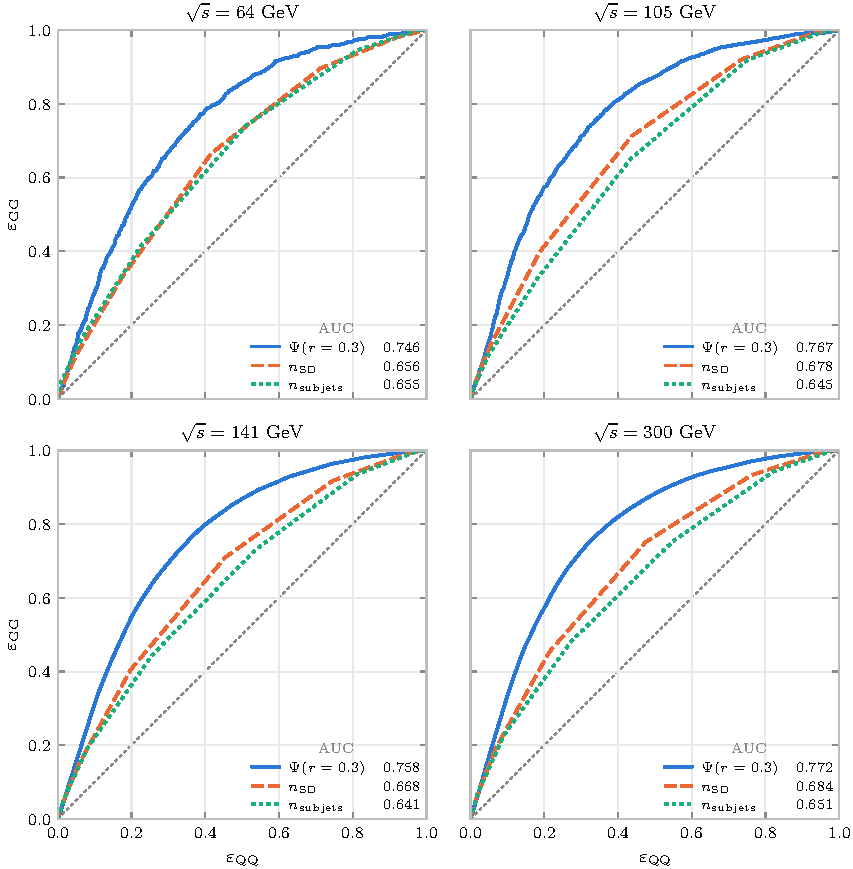
\includegraphics[width=0.46\textwidth]{figs/fig_roc_panels.pdf}

\vspace{-0.3em}
\flushleft\footnotesize
\begin{tabular}{lcccc}
\toprule
$\sqrt{s}$ [GeV] & 64 & 105 & 141 & 300 \\
\midrule
\psic{$\Psi(0.3)$}        & 0.746 & 0.767 & 0.758 & \textbf{0.772} \\
\sdc{$n_{\mathrm{SD}}$}   & 0.656 & 0.678 & 0.668 & 0.684 \\
\sjc{$n_{\mathrm{subjets}}$} & 0.655 & 0.645 & 0.641 & 0.651 \\
\bottomrule
\end{tabular}

\vspace{0.6em}
\normalsize
In practice: at 20\% quark contamination, $\Psi$ keeps \textbf{twice as many}
gluon jets as $n_{\mathrm{subjets}}$.

\end{frame}

% ===================================================================
\begin{frame}{Why the simplest observable wins}

Both counting observables boil the jet down to \emph{how many splittings clear
a threshold}. Everything below the threshold is thrown away.

\vspace{0.8em}
At EIC energies a 10--20~GeV jet has only \textbf{three or four} splittings
that qualify. You are counting on a very coarse ruler.

\vspace{0.8em}
Our own data says so. Theory predicts the gluon/quark ratio of
$n_{\mathrm{SD}}$ should approach $C_A/C_F = 2.25$. We measure:
\[
\frac{\langle n_{\mathrm{SD}}\rangle_{\mathrm{GG}}}
     {\langle n_{\mathrm{SD}}\rangle_{\mathrm{QQ}}}
= \frac{4.41}{3.47} = 1.27
\]
Barely half the asymptotic value. The counting argument is \emph{not sharp}
here.

\vspace{0.8em}
$\Psi(r)$ throws nothing away --- every constituent contributes, weighted by
its energy.

\vspace{0.8em}
\centering\textbf{When there is little to count, don't count.}

\end{frame}

% ===================================================================
\begin{frame}{Result 2: $\Psi(0.3) < 0.6$ was a good choice}

The companion paper picked its thin/thick cut by eye, years ago. Was that
lucky or right?

\vspace{1em}
\centering
\begin{tabular}{lcc}
\toprule
cut on $\Psi(0.3)$ & gluons kept & quarks let in \\
\midrule
$< 0.60$ \quad\textcolor{gray}{(the paper's choice)} & 0.712 & 0.289 \\
$< 0.63$ \quad\textcolor{gray}{(the optimum)}        & 0.758 & 0.329 \\
\bottomrule
\end{tabular}

\vspace{1.2em}
\flushleft
Sweeping every possible cut and asking which maximises
$\varepsilon_{\mathrm{GG}} - \varepsilon_{\mathrm{QQ}}$ gives
\textbf{0.63}.

\vspace{0.6em}
The paper chose \textbf{0.60}.

\vspace{1.2em}
\centering
\textbf{Essentially optimal} --- within $0.03$ of the best available cut.

\vspace{1em}
\flushleft\footnotesize
The other cut, $\Psi > 0.8$ for quark-like jets, reads in reverse: it keeps
37\% of quark jets while admitting only 6\% of gluon jets. A small but very
clean quark sample.

\end{frame}

% ===================================================================
\begin{frame}{Result 3: the counting observables swap places}

\textbf{Pooled over $\eta$:} \sdc{$n_{\mathrm{SD}}$} beats
\sjc{$n_{\mathrm{subjets}}$}. That is what the literature predicts.

\vspace{0.8em}
\textbf{Binned in $\eta$:} \sjc{$n_{\mathrm{subjets}}$} wins --- in
\textbf{all fourteen bins}, at every energy, no exceptions, by 0.027 to 0.072.

\vspace{1em}
\centering
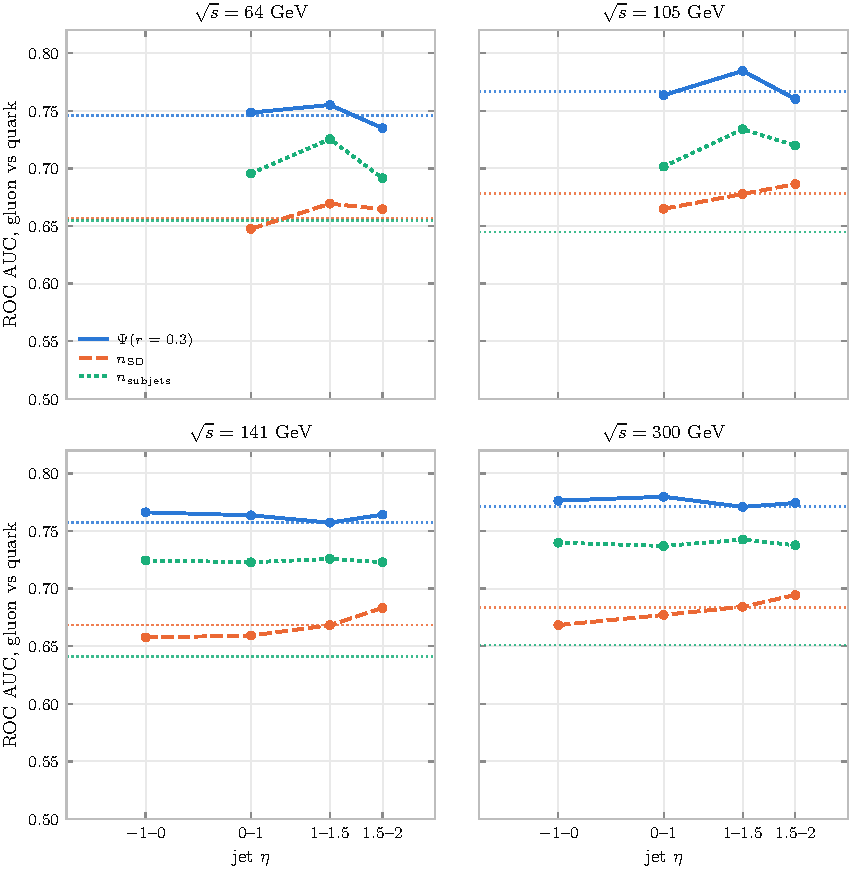
\includegraphics[width=0.52\textwidth]{figs/fig_auc_vs_eta.pdf}

\vspace{-0.2em}
\flushleft\footnotesize
Dotted lines are the pooled values. \psic{$\Psi$} and \sdc{$n_{\mathrm{SD}}$}
sit on theirs. \sjc{$n_{\mathrm{subjets}}$} floats far above its own.

\end{frame}

% ===================================================================
\begin{frame}{An analogy for what is going wrong}

Imagine ranking students by raw exam score --- but different schools set
papers of different difficulty.

\vspace{1em}
\begin{itemize}
  \item \textbf{Within one school}, the ranking works fine.
  \item \textbf{Pool all schools}, and you mostly measure \emph{which school
        they attended}, not who is better.
\end{itemize}

\vspace{1.5em}
That is exactly what happens to $n_{\mathrm{subjets}}$ across $\eta$.

\vspace{1em}
Its mean slides from \textbf{4.25} in the most backward bin to \textbf{2.49}
in the most forward one. A gluon jet out front looks like a quark jet in the
middle.

\vspace{1em}
Splitting the pooled variance: \textbf{27--39\%} of the width of
$n_{\mathrm{subjets}}$ is this sliding, not class information. For
$n_{\mathrm{SD}}$ it is \textbf{0.2\%}.

\end{frame}

% ===================================================================
\begin{frame}{See it directly}

\centering
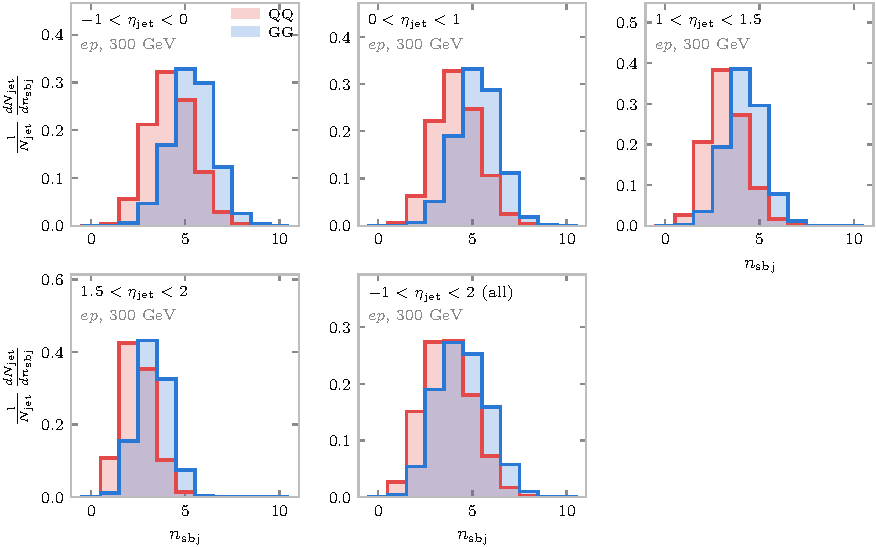
\includegraphics[width=0.70\textwidth]{figs/dist_nsubjets_hera300_antikt_dijets.pdf}

\vspace{-0.2em}
\flushleft\footnotesize
\sjc{$n_{\mathrm{subjets}}$}: the whole distribution marches \emph{left} as
$\eta$ grows --- peak at 5, then 5, then 4, then 3. The last panel pools them
all: broader, flatter, far more overlap. The QQ--GG shift drops to 0.75,
\emph{smaller than in any individual bin}.

\end{frame}

% ===================================================================
\begin{frame}{The same plot for $n_{\mathrm{SD}}$}

\centering
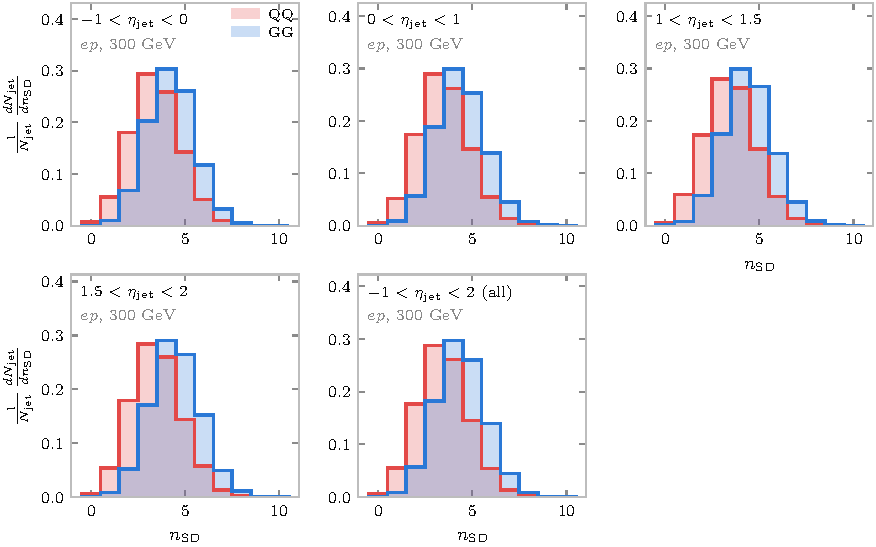
\includegraphics[width=0.70\textwidth]{figs/dist_nsd_hera300_antikt_dijets.pdf}

\vspace{-0.2em}
\flushleft\footnotesize
\sdc{$n_{\mathrm{SD}}$}: nothing moves. Every panel looks the same, and the
pooled panel looks like the others --- because there is nothing to smear.

\vspace{0.5em}
\centering\normalsize
\textbf{Two observables, same jets. One has a problem the other does not.}

\end{frame}

% ===================================================================
\begin{frame}{The physics: a moving ruler}

It is natural to read $n_{\mathrm{subjets}}$ as counting above a \emph{fixed
momentum scale}. In the implementation we use, it does not.

\vspace{0.6em}
The $y_{\mathrm{cut}}$ is normalised to the summed constituent
\textbf{energy}:
\[
\min(p_{T,i}, p_{T,j})\,\Delta R_{ij} \;>\; \sqrt{y_{\mathrm{cut}}}\;E_{\mathrm{jet}}
\]

Write $p_T = z\,p_T^{\mathrm{jet}}$ and $E = p_T^{\mathrm{jet}}\cosh\eta$.
The jet $p_T$ \textbf{cancels}, leaving
\[
\boxed{\;z\,\Delta R \;>\; \sqrt{y_{\mathrm{cut}}}\;\cosh\eta\;}
\]

\vspace{0.6em}
So the effective threshold \emph{grows as you go forward}:

\centering
\begin{tabular}{lccc}
\toprule
$\eta$ & 0.0 & 1.5 & 2.5 \\
\midrule
$z_{\mathrm{eff}}$ & 0.022 & 0.053 & \textbf{0.137} \\
\bottomrule
\end{tabular}

\vspace{0.6em}
\flushleft
while \sdc{$n_{\mathrm{SD}}$} cuts at $z > 0.1$ \emph{everywhere}.

\end{frame}

% ===================================================================
\begin{frame}{Three ways we checked it}

\textbf{1. Energy, not $p_T$, is what it responds to.}\\
\footnotesize
Binned in jet energy: $\langle n_{\mathrm{subjets}}\rangle$ falls
$4.23 \rightarrow 1.50$. $\langle n_{\mathrm{SD}}\rangle$ holds at
$3.43$--$3.50$.

\vspace{1em}
\normalsize
\textbf{2. The functional form is exactly right.}\\
\footnotesize
Counting grows like $\ln(1/z)$, so the count should fall linearly in
$\ln\cosh\eta$. Measured at fixed $p_T$:
\[
\langle n_{\mathrm{subjets}}\rangle = 4.35 - 1.53\,\ln\cosh\eta,
\qquad r^2 = 0.991
\]

\vspace{0.8em}
\normalsize
\textbf{3. It predicted a crossover we had not measured.}\\
\footnotesize
$z_{\mathrm{eff}}$ passes $0.1$ near $\eta \approx 2.2$, so beyond that
$n_{\mathrm{SD}}$ should retake the lead. Extending the bins:

\centering
\begin{tabular}{lccc}
\toprule
$\eta$ bin & [1.5, 2) & [2.5, 3) & [3, 4) \\
\midrule
\sdc{$n_{\mathrm{SD}}$}      & 0.694 & \textbf{0.694} & \textbf{0.698} \\
\sjc{$n_{\mathrm{subjets}}$} & \textbf{0.738} & 0.682 & 0.550 \\
\bottomrule
\end{tabular}

\vspace{0.5em}
Predicted 2.2. Observed between 2.25 and 2.75.

\end{frame}

% ===================================================================
\begin{frame}{So which counter is actually better?}

\textbf{$n_{\mathrm{subjets}}$ is --- where its threshold is soft.}

\vspace{0.8em}
Centrally it resolves emissions about \textbf{five times softer} than
$n_{\mathrm{SD}}$ ($z \approx 0.022$ against $0.1$), so it samples far more of
the Casimir-weighted radiation. More information per jet.

\vspace{1.2em}
Its weakness is not the counting. It is the \textbf{moving threshold}.

\vspace{0.8em}
Pooled across $\eta$, the same observable is effectively a different
measurement in each part of the range --- so the classes smear together.

\vspace{1.5em}
\hrule
\vspace{0.8em}
\textbf{Practical upshot:}
\begin{itemize}
  \item Quoting \emph{inclusively}? Use $n_{\mathrm{SD}}$.
  \item Quoting \emph{differentially in $\eta$}? Use $n_{\mathrm{subjets}}$.
  \item Or fix it at source: scale $y_{\mathrm{cut}}$ by $1/\cosh^2\eta$,
        or recluster in a frame where the jet is central.
\end{itemize}

\end{frame}

% ===================================================================
\begin{frame}{What we recommend}

\textbf{For the first generation of EIC jet-substructure measurements, use the
integrated jet shape $\Psi(r)$.}

\vspace{1em}
\begin{itemize}
  \item Best separation of the three, at every energy
  \item Flat across the whole EIC range, and matches the HERA reference
  \item \textbf{No tagging parameter beyond the choice of $r$} --- and $r$ is
        less a knob than a choice of where to read a profile measured in full
  \item Directly comparable to archival ZEUS measurements. (So is
        $n_{\mathrm{subjets}}$, by construction; $n_{\mathrm{SD}}$ has no $ep$
        measurement to check against)
\end{itemize}

\vspace{1.2em}
\textbf{And a concrete warning:} do not quote $n_{\mathrm{subjets}}$
inclusively over a wide $\eta$ range without saying so. Its discrimination
power is real, but pooling throws much of it away.

\end{frame}

% ===================================================================
\begin{frame}{Honest limits}

\begin{itemize}
  \item \textbf{Generator level only.} No detector effects. The comparison is
        relative, so smearing should hit all three similarly --- but we have
        not shown that.
  \item \textbf{Three observables, not the landscape.} Angularities, energy-flow
        polynomials and energy correlators are not here.
  \item \textbf{No statistical uncertainties quoted on the AUCs.} Two jets from
        one event are correlated, so honest error bars need bootstrapping over
        \emph{events}, not jets.
  \item \textbf{The $1/\cosh^2\eta$ fix is suggested, not tested.}
\end{itemize}

\vspace{1.5em}
\centering
\large
What does not change: \psic{$\Psi(r=0.3)$} wins at every energy,
in every $\eta$ bin, at every bin width.

\end{frame}

% ===================================================================
\begin{frame}{One-slide summary}

\begin{enumerate}
  \item A ROC curve is built by sliding a \textbf{pass mark} through every
        possible value and recording two numbers each time: gluons kept,
        quarks let in.
  \vspace{0.4em}
  \item The \textbf{AUC} is the area underneath --- the chance a random gluon
        jet outscores a random quark jet. It contains no choice of cut.
  \vspace{0.4em}
  \item \psic{$\Psi(0.3)$} wins at every energy (0.75--0.77), because counting
        observables have too little to count at 10--20~GeV.
  \vspace{0.4em}
  \item The companion paper's cut at \textbf{0.6} is essentially the optimum
        (0.63). Good call.
  \vspace{0.4em}
  \item \sjc{$n_{\mathrm{subjets}}$} and \sdc{$n_{\mathrm{SD}}$} swap places
        depending on whether you pool or bin in $\eta$ ---
        because the $k_T$ threshold is normalised to \emph{energy}, so it
        tightens as $\cosh\eta$.
\end{enumerate}

\end{frame}

\end{document}
